\documentclass[a4paper,10pt]{article}
\usepackage{dsfont}
\usepackage{bbold}
\usepackage{stmaryrd}
\usepackage{mathrsfs}
\usepackage{fancyhdr}
\usepackage{algorithm,algpseudocode}
\usepackage{graphicx}
%% %%%%%%%%%%%%%%%%%%%%%%%%%%%%%%%%%%%%%%%%%%%%%%%%%%%%%%%%%%%%%%%%%%%%%%%%%%%%%
%% %%%%%%% %% %% %  %                                      %  % %% %% %%%%%%%%%%
%%%%% %% %  %                    MES COMMANDES                     %  % %% %%%%%
%%%%%%%%%% %% %% %  %                                      %  % %% %% %%%%%%% %%
%%%%%%%%%%%%%%%%%%%%%%%%%%%%%%%%%%%%%%%%%%%%%%%%%%%%%%%%%%%%%%%%%%%%%%%%%%%%% %%


\newcommand{\zzpackages}[1][french]{
  \usepackage[utf8]{inputenc}
  \usepackage[T1]{fontenc}
  \usepackage[#1]{babel}

  \usepackage{amsthm}
  \usepackage{amsmath}
  \usepackage{amsfonts}
  \usepackage{amssymb}

  \usepackage{xcolor}
  \usepackage{xstring}	%\ifstreqcase
}

%% %%%%%%%%%%%%%%%%%%%%%%%%%%%%%%%%%%%%%%%%%%%%%%%%%%%%%%%%%%%%%%%%%%%%%%%%%%%%%
%                              TESTS / FOR / ...                               %
%%%%%%%%%%%%%%%%%%%%%%%%%%%%%%%%%%%%%%%%%%%%%%%%%%%%%%%%%%%%%%%%%%%%%%%%%%%%% %%

% 
\def\defactive#1#2{
  \catcode`#1=13
  \begingroup
  \lcode`~=`#1
  \lowercase{\endgroup\def~}{#2}
}

\def\zifempty#1#2#3{\def\foo{#1}\ifx\foo\empty\relax#2\else#3\fi}

%% %%%%%%%%%%%%%%%%%%%%%%%%%%%%%%%%%%%%%%%%%%%%%%%%%%%%%%%%%%%%%%%%%%%%%%%%%%%%%
%                           MARGES / HYPERREF / ...                            %
%%%%%%%%%%%%%%%%%%%%%%%%%%%%%%%%%%%%%%%%%%%%%%%%%%%%%%%%%%%%%%%%%%%%%%%%%%%%% %%

\makeatletter
\gdef\@subtitle{}
\def\subtitle#1{\gdef\@subtitle{#1}}

\def\zztitre{
\begingroup\centering
{\bfseries \huge \@title}\par\vspace{.3cm}
\ifx\@subtitle\empty\else{\bfseries \Large \@subtitle}\par\vspace{.5cm}\fi
\Large \@author\par\vspace{.1cm}
\@date\zal\vspace{.3cm}\zal
\zligne\endgroup
}

\makeatother


\newcommand{\zzhyperref}{
\usepackage{hyperref}
\hypersetup{ colorlinks=true, linkcolor=blue!30!black,
citecolor=green!30!black, filecolor=magenta!30!black,
urlcolor=cyan!30!black }
}

\newcommand{\zzmarges}{
  \setlength{\textheight}{620pt}
  \addtolength{\textwidth}{2cm}
  \addtolength{\hoffset}{-1cm}
  \addtolength{\voffset}{-1cm}
  \addtolength{\marginparwidth}{0cm}
  \addtolength{\textheight}{1cm}
} 

\makeatletter
\newcommand{\zzheader}[6]{
\def\@oddhead{\vbox to 0pt{\vss\hspace{0pt} #1\hfill #2\hfill #3\kern4pt\par\kern5pt\hrule height.5pt}}
\def\@oddfoot{\vbox to 0pt{\hrule height.5pt\kern5pt\hbox to \linewidth{\kern4pt {#4}\hss {#5}\hss {#6}\kern4pt}\vss}}}
\makeatother

%%%%%%%%%%%%%%%%%%%%%%%%%%%%%%%%%%%%%%%%%%%%%%%%%%%%%%%%%%%%%%%%%%%%%%%%%%%%%%%%

\newcommand{\zligne}[1][]{
\par\zifempty{#1}%
{\hbox to \linewidth{\leaders\hrule height3pt depth-2.5pt\hfill}}%
{\hbox to \linewidth{\leaders\hrule height3pt depth-2.5pt\hfill\kern.8em #1\kern.8em\leaders\hrule height3pt depth-2.5pt\hfill}}\par
}

%%%%%%%%%%%%%%%%%%%%%%%%%%%%%%%%%%%%%%%%%%%%%%%%%%%%%%%%%%%%%%%%%%%%%%%%%%%%%%%%

\newcommand{\zal}{\par}
\newcommand{\znl}{\zal ~\zal}
\newcommand{\zguill}[2][]{«\,#2\,»}

%% %%%%%%%%%%%%%%%%%%%%%%%%%%%%%%%%%%%%%%%%%%%%%%%%%%%%%%%%%%%%%%%%%%%%%%%%%%%%%
%                             COMMANDES PRATIQUES                              %
%%%%%%%%%%%%%%%%%%%%%%%%%%%%%%%%%%%%%%%%%%%%%%%%%%%%%%%%%%%%%%%%%%%%%%%%%%%%% %%

%% ------- -- -- -  -                                      -  - -- -- --------%%
%---- -- -  -                          ZP                          -  - -- ----%
%%-------- -- -- -  -                                      -  - -- -- ------- %%
\makeatletter
\def\z@first#1#2{#1}
\def\z@second#1#2{#2}
\def\z@zp@selectchar#1#2{
  \IfStrEqCase{#2}{%
    {p}{#1{(}{)}}%
    {c}{#1{[}{]}}%
    {a}{#1{\{}{\}}}%
    {C}{#1{]}{[}}%
    {b}{#1{|}{|}}%
    {n}{#1{\|}{\|}}%
    {i}{#1{[}{]}\!#1{[}{]}}%
    {t}{#1{<}{>}}%
    {v}{#1{.}{.}}%
    {A}{#1{\}}{\{}}%
    {P}{#1{)}{(}}%
    {I}{#1{]}{[}\!#1{]}{[}}%
    {T}{#1{>}{<}}%
  }[#1{(}{)}]%
}

\def\z@zp#1#2\fin#3{
  \z@zp@selectchar{\left\z@first}{#1}#3
  \zifempty{#2}%
        {\z@zp@selectchar{\right\z@second}{#1}}%
        {\z@zp@selectchar{\right\z@second}{#2}}%
}
\newcommand{\zp}[2][]{\zifempty{#1}{\left(#2\right)}{\z@zp#1\fin{#2}}}

\newcommand{\zpbig}[1]{\ifcase#1\relax\vrule width0pt height0pt\or\vrule width0pt height9pt\or\vrule width0pt height10pt\or\vrule width0pt height13pt\else\vrule width0pt height16pt\fi}

%% ------- -- -- -  -                                      -  - -- -- --------%%
%---- -- -  -                   Itemize et autre                   -  - -- ----%
%%-------- -- -- -  -                                      -  - -- -- ------- %%

\newcommand{\zitemize}[1]{
\vspace{-\topsep}\begin{itemize}\setlength\itemsep{0pt plus 1pt}\setlength\parskip{0cm}#1\end{itemize}\vspace{-\topsep}}


%% ------- -- -- -  -                                      -  - -- -- --------%%
%---- -- -  -                        AUTRES                        -  - -- ----%
%%-------- -- -- -  -                                      -  - -- -- ------- %%

\newcommand{\zR}{\mathbb{R}}

\newcommand{\zsum}[2][0pt]{\sum_{\hbox to #1{\hss$\scriptstyle#2$\hss}}}
\newcommand{\zprod}[2][0pt]{\prod_{\hbox to #1{\hss$\scriptstyle#2$\hss}}}

\newcommand{\zseq}[1][=]{\hspace{2pt}\raise .5pt\hbox{\scalebox{.8}{#1}}\hspace{2pt}}

\newcommand{\zop}[2]{\mathrm{#1}\zp{#2}}

\newcommand{\zi}{\mathrm{i}}

\newcommand{\zexp}[1]{\mathrm{e}^{#1}}

\newcommand{\zmatrix}[2]{\left(\begin{array}{#1}#2\end{array}\right)}

\newcommand{\zindic}[1]{%
\hbox to 5.3pt{1\hss l}\hskip -2.5pt\left\{#1\right\}%
}

\newcommand{\zesp}[2][]{%              esperance
\mathbb{E}_{#1}\hskip -3pt\left[\zpbig1\,#2\,\right]%
}

\newcommand{\zprob}[2][]{%             proba
\mathbb{P}_{#1}\hskip -3pt\left(\zpbig1\,#2\,\right)%
}

% Symbole d'indépendance de variable aléatoire
\newcommand{\zindep}{\protect\mathpalette{\protect\z@ind}{\perp}}
\def\z@ind#1#2{\mathrel{\rlap{$#1#2$}\mkern6mu{#1#2}}}


\newcommand{\zdx}[1]{\mathrm{d}#1}

\newcommand{\zderiv}[2]{\frac{\partial #1}{\partial #2}}


\newcommand{\ztr}[2][]{\zifempty{#1}{#2}{\left(#2\right)}^{\hspace{-1pt}\mathsf{T}}\hspace{-1pt}}
\def\zpreind#1#2{ \raise-.35ex\hbox{\scriptsize$#1$}#2}
\def\zpreexp#1#2{ \raise.85ex\hbox{\scriptsize$#1$}#2}

%% %%%%%%%%%%%%%%%%%%%%%%%%%%%%%%%%%%%%%%%%%%%%%%%%%%%%%%%%%%%%%%%%%%%%%%%%%%%%%
%                                 ALGORITHMES                                  %
%%%%%%%%%%%%%%%%%%%%%%%%%%%%%%%%%%%%%%%%%%%%%%%%%%%%%%%%%%%%%%%%%%%%%%%%%%%%% %%

\newcount\z@algo@count
\newdimen\z@algo@indent
\begingroup
  \catcode`\^^M=13             %
  \catcode`\^^I=13             %
  \gdef\z@algo{                %
  \z@algo@count=1
    \begingroup                %
    \catcode`\^^M=13           %
    \def^^M{\leavevmode\par \advance\z@algo@count by 1\z@algo@indent=0pt}%
    \catcode`\^^I=13           %
    \def^^I{\advance\z@algo@indent by 1em}         %
    \everypar{                 %
      \hbox to 0cm{\hss\textcolor{black!30}{\the\z@algo@count~:}}~\kern\z@algo@indent}  %
                               %
    \tt                        %
  }

\endgroup

\newenvironment{zalgo}{\z@algo}{\endgroup}


\makeatother



%% %%%%%%%%%%%%%%%%%%%%%%%%%%%%%%%%%%%%%%%%%%%%%%%%%%%%%%%%%%%%%%%%%%%%%%%%%%%%%
%                                    AUTRE                                     %
%%%%%%%%%%%%%%%%%%%%%%%%%%%%%%%%%%%%%%%%%%%%%%%%%%%%%%%%%%%%%%%%%%%%%%%%%%%%% %%

% epaisseur trait / marge / texte

\def\zfbox#1#2#3{
  \hbox{\vrule width #1
    \vtop{
      \vbox{
        \hrule height #1
        \kern #2
        \hbox{\kern #2 #3\kern #2}
      }%
      \kern #2%
      \hrule height #1
    }%
    \vrule width #1%
  }%
}

%% \begin{mygraph}{xmin=0, xmax=1, %
%%                ymin=0, ymax=1, %
%%                sizex=2.5, sizey=2.5}%
%%                {nomx=Axe X, nomy=Axe Y}%
%%                {0,.5,1}{0,0.25,...,1.05}

%% \graduationX[dashed, blue]{ .78 / $\frac{\pi}{4}$ }{ PARAMETRE TEXT }

%% \begin{mylegend}{x=0.3, y=.9, n=2, t=2.1, scale=.5}
%%   \newlegend{blue}{Courbe 1}
%%   \newlegend{red}{Courbe 2}
%% \end{mylegend}

%% \fillbetweencurve[opacity=.2, blue]{ COURBE 1 }{ COURBE 2 }

%% \end{mygraph}


\usepackage{tikz}



\pgfkeys{
%
 /mygraph/.is family, /mygraph,
 xmin/.estore in = \xn,
 xmax/.estore in = \xm,
 ymin/.estore in = \yn,
 ymax/.estore in = \ym,
 sizex/.estore in = \xx,
 sizey/.estore in = \yy,
 %
/mygraphb/.is family, /mygraphb,
 nomx/.estore in = \axex,
 nomy/.estore in = \axey,
%
/mygraphc/.is family, /mygraphc,
 gradsize/.estore in = \gradsize,
 gradsize/.default = 0.1,
 nomydist/.estore in = \axeyd,
 nomydist/.default = 0.8cm,
 gradsize, nomydist,                 % NE PAS OUBLIER
%
/myleg/.is family, /myleg,
 x/.estore in = \legendx,
 y/.estore in = \legendy,
 n/.estore in = \legendn,
 t/.estore in = \legendt,
 scale/.estore in = \legends,
 scale/.default = 1,
 scale,
%
/mylego/.is family, /mylego,
size/.estore in = \legendwidth,
size/.default = 0.4,
size                                  % NE PAS OUBLIER
}


%%%%%%%%%%%%%%%%%%%%%%%%%%%%%%%%%%%%%%%%%%%%%%%%%%%%%%%%%%%%%%%%%%%%%%%%%%%%%%%%
%                                                                              %
%%%%%%%%%%%%%%%%%%%%%%%%%%%%%%%%%%%%%%%%%%%%%%%%%%%%%%%%%%%%%%%%%%%%%%%%%%%%%%%%

\newenvironment{mygraph}[5][]{%
\pgfkeys{/mygraph, #2}
\pgfkeys{/mygraphb, #3}
\pgfkeys{/mygraphc, #1}
  \pgfmathsetmacro\dum{\yy/(\ym-\yn)}
  \pgfmathsetmacro\dumm{\xx/(\xm-\xn)}
\begin{tikzpicture}[yscale=\dum, xscale=\dumm,font=\sffamily]
  \pgfmathsetmacro\gradx{\gradsize / \dum}
  \pgfmathsetmacro\grady{\gradsize / \dumm}

  \foreach \x in {#4}{
    \draw[very thin, color=black, dotted] (\x,\yn) -- (\x,\ym);
    \draw (\x,\yn+\gradx) -- (\x,\yn)
          node[font=\tiny, anchor=north] {\pgfmathprintnumber{\x}};
  };
  \foreach \y in {#5}{
    \draw[very thin, color=black, dotted] (\xn,\y) -- (\xm,\y); 
    \draw (\xn+\grady,\y) -- (\xn,\y)
          node[font=\tiny, anchor=east] {\pgfmathprintnumber{\y}};
  };
  \draw (\xn,\yn) -- node[font=\scriptsize, below=0.3cm] {\axex} (\xm,\yn);
  \draw (\xn,\yn) -- node[font=\scriptsize, rotate=90, above=\axeyd, anchor=mid] {\axey} (\xn,\ym);
  \draw (\xn,\ym) -- (\xm,\ym);
  \draw (\xm,\yn) -- (\xm,\ym);

  \begin{scope}
    \clip (\xn,\yn) rectangle (\xm,\ym);
    %% \draw[dashed] (\xn, 0) -- (\xm, 0);
    %% \draw[dashed] (0, \yn) -- (0, \ym);
}{
  \end{scope}
\end{tikzpicture}
}

%%%%%%%%%%%%%%%%%%%%%%%%%%%%%%%%%%%%%%%%%%%%%%%%%%%%%%%%%%%%%%%%%%%%%%%%%%%%%%%%

\newenvironment{mylegend}[2][]{
\pgfkeys{/myleg, #2}
\pgfkeys{/mylego, #1}
\begin{scope}[shift={(\legendx,\legendy)}, scale=\legends]
\pgfmathsetmacro\legendwidth{\legendwidth * (\xm-\xn) / \xx }
\pgfmathsetmacro\dum{ (0.125 * (\ym-\yn) / \yy) }
\pgfmathsetmacro\dumm{ - (0.125 * (\xm-\xn) / \xx) }
\pgfmathsetmacro\legendy{ 0 }
\coordinate (dum) at (\dumm,\dum);
\pgfmathsetmacro\dum{ - (\legendn-0.4)*(0.25 * (\ym-\yn) / \yy) }
\coordinate (dumm) at (\dumm,\dum);
\pgfmathsetmacro\dumm{\dumm + (\legendt * (\xm-\xn) / \xx) }
\draw[fill=white, opacity=.8] (dum) -- (dumm) -| (\dumm,\dum) |- (dum);
}{
\end{scope}
%% \pgfmathsetmacro\legendyi{\legendyi + (0.125 * (\ym-\yn) / \yy)  }
%% \pgfmathsetmacro\legendy{\legendy + (0.1 * (\ym-\yn) / \yy)  }
%% \pgfmathsetmacro\legendx{\legendx - (0.125 * (\xm-\xn) / \xx)  }
%% \draw[] (\legendx,\legendyi) -- (\legendx,\legendy) %
%%                              -| (\legendx + 1,\legendy)
%%                              |- (\legendx,\legendyi);
}

\newcommand{\newlegend}[2]{
\draw[font=\scriptsize, #1] (0,\legendy) -- (\legendwidth,\legendy)	node[right,scale=\legends]{#2};
\pgfmathsetmacro\legendy{\legendy - (0.25 * (\ym-\yn) / \yy)  }
}

%%%%%%%%%%%%%%%%%%%%%%%%%%%%%%%%%%%%%%%%%%%%%%%%%%%%%%%%%%%%%%%%%%%%%%%%%%%%%%%%

\newenvironment{outofbox}{%
  \end{scope}%
}{%
  \begin{scope}%
    \clip (\xn,\yn) rectangle (\xm,\ym);%
}

%%%%%%%%%%%%%%%%%%%%%%%%%%%%%%%%%%%%%%%%%%%%%%%%%%%%%%%%%%%%%%%%%%%%%%%%%%%%%%%%

\newcommand{\fillbetweencurve}[3][]{
\begin{scope}
\clip (\xn,\yn) -- #2 -- (\xm,\yn) -- cycle;
\fill[#1] (\xn,\ym) -- #3 -- (\xm,\ym) -- cycle;
\end{scope}
}

%%%%%%%%%%%%%%%%%%%%%%%%%%%%%%%%%%%%%%%%%%%%%%%%%%%%%%%%%%%%%%%%%%%%%%%%%%%%%%%%

\newcommand{\graduationX}[3][very thin, color=black, dotted]{
\end{scope}
  \foreach \x/\t in {#2}{
    \draw[#1] (\x,\yn) -- (\x,\ym);
    \draw (\x,\yn+\gradx) -- (\x,\yn)
          node[font=\tiny, anchor=north, #3] {\t};
  };
\begin{scope}%
\clip (\xn,\yn) rectangle (\xm,\ym);%
}

%%%%%%%%%%%%%%%%%%%%%%%%%%%%%%%%%%%%%%%%%%%%%%%%%%%%%%%%%%%%%%%%%%%%%%%%%%%%%%%%

\newcommand{\graduationY}[3][very thin, color=black, dotted]{
\end{scope}
  \foreach \y/\t in {#2}{
    \draw[#1] (\xn,\y) -- (\xm,\y);
    \draw (\xn+\grady,\y) -- (\xn,\y)
          node[anchor=east, font=\tiny, shift={(-0*\grady,0)}, #3] {\t};
  };
\begin{scope}%
\clip (\xn,\yn) rectangle (\xm,\ym);%
}

\zzpackages[english]

\tikzset{
zplot/.style={opacity=.8}
}

\begin{document}

\title{MVA Reinforcement Learning\\
Optimization of very difficult functions}

\author{Nathan de Lara, Florian Tilquin}
%\date{}
\maketitle

\section{Introduction}
\subsection{Problem statement}
The goal of this paper is to test and compare recently developed algorithms for the optimization of \textit{very difficult functions}. This work is based on the papers by Bubeck~\cite{bubeck2011x}, Grill~\cite{grill2015black}, Lazaric~\cite{azar2014online}, Bull~\cite{bull2013adaptive} and Valko~\cite{valko2013stochastic}. Each one of this paper has a specific definition of \textit{difficult} but the general idea is that the function to optimize has many local maxima and only one global maximum, it has very fast variations and is not necessarily differentiable such that a gradient-based approach to find the optimum should not be successful. All functions are assumed to be bounded and to have a compact support which, up to scaling can be fixed to be $[0,1]^p$. In this paper, we only consider $p=1$. In the end, the general formulation of the problem is:
\begin{equation}
\mbox{maximize } f(x) \mbox{ for } x\in [0,1]
\end{equation}

\subsection{About the multi-armed bandit}
\label{mab}
As previously mentioned, a gradient-based approach is not likely to perform well on the considered functions. Thus, the idea is to use a multi-armed bandit with theoretically an infinite number of arms, sometimes called \textit{continuum-armed bandit}. The algorithms progressively defines a sequence of evaluation points $x_t$ and observes a reward $y_t=f(x_t)+\xi_t$ where $\xi_t$ is a noise term. The choice of $x_{t+1}$ depends on the sequence of $(y_{t'})_{t'\le t}$. Depending on the algorithm, it is meant to converge to $x^*$ while controlling the cumulative regret:
\begin{equation}
\label{regret}
R_T = \underset{t=1}{\overset{T}{\sum}}f(x^*)-f(x_t)
\end{equation}
Or just simply ensuring that a good estimate of $x^*$ is present in the sequence (i.e minimizing simple regret). They can also be designed to be robust to noise in function estimations or correlated feedback. This design depends on the optimization context: is it an off-line or online optimization ? how long does an evaluation of the function take? etc.\\
In practice, for the algorithms considered, $x_t = \mathcal{U}(I_t)$. This means that $x_t$ is pulled uniformly at random in an interval $I_t$ that is chosen by the algorithm. The set of intervals defines a tree structure such that the set of leaves is a partition of $[0,1]$. In the end, the original problem is transformed into a particular case of regular multi-armed bandit. Without any prior information on the function to optimize, we only consider here the family of \textit{dyadic trees}. As mentioned in~\cite{bull2013adaptive}, the dyadic tree on [0, 1) is the tree with root node [0, 1), and where each node [a, b) has children $[a, \frac{1}{2}(a+b), [ \frac{1}{2}(a+b), b)$. An example of dyadic tree is displayed in~\ref{dydtree}. 

\begin{figure}
\label{dydtree}
\centering
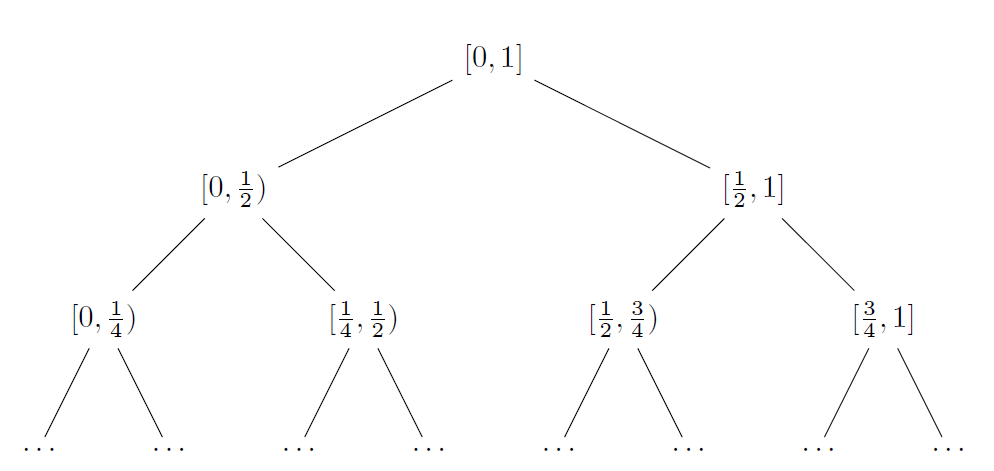
\includegraphics[scale=0.3]{dyadic}
\caption{A dyadic tree from~\cite{bull2013adaptive}}
\end{figure}

\subsection{Notations}
In the rest of this paper, we note:
\begin{itemize}
\item $h,i$ the coordinates of a node in the dyadic tree such that $h$ is the depth of the node and $i$ its width
\item $\widehat{\mu}_{h,i}$ the empirical estimate of the reward associated to the node $h,i$
\item $n_{h,i}$ the number of times the node $h,i$ has been hit during the evaluations up to the current time
\item $T_{max}$ the total number of evaluations of the function allowed or \textit{budget}
\end{itemize} 



\section{Algorithms}
\label{algo}
In this section, we list the algorithms to be compared and briefly present their respective behaviors. The reader is welcome to consult the original papers for more detailed descriptions and proofs on theoretical performances. As previously mentioned, each algorithm defines a sequence of intervals $I_t$ from which $x_t$ is sampled. Typically, the selected interval maximizes a certain selection function of $(x_{t'},y_{t'})_{t'< t}$ among a subset of considered intervals. The main differences in the following algorithms is the definition of the selection function, which is most of the time an upper bound on the expected reward of the arm and the choice of the considered intervals at each time step, which is sometimes called "expansion rule".

\subsection{Hierarchical and Parallel Optimistic Optimization}
This algorithm is called \textit{Optimistic} because its idea is to sequentially building a tree and try the most promising children.
\paragraph{Upper bounds} $B_{h,i}=min(U_{h,i},max(B_{h+1,2i-1},B_{h,2i}))$ where:
\begin{equation}
\label{uhoo}
U_{h,i}=\widehat{\mu}_{h,i}+\nu \rho^h+\sqrt{\dfrac{2\log(T_{max})}{n_{h,i}}}
\end{equation}
\paragraph{Update rule} At each time step, the most promising child with respect to B is added to the tree.

\paragraph{Parallel Optimistic Optimization}
When there is no prior knowledge on the function to optimize, the tuning of the parameters $\nu$ and $\rho$ of equation~\ref{uhoo} can be difficult. Thus, the idea of this algorithm is to sequentially launch several HOOs that keep running in parallel in order to get the best parameters. Note that this algorithm can be run with other algorithms than HOO such as HCT.

\subsection{High-Confidence Tree}
This algorithm exists in two different versions: with correlated and uncorrelated feedback. For the purpose of performance comparison with other algorithms, we only consider the uncorrelated feedback, which is close to HOO algorithm. In order to be pulled, an arm must maximize $B$ among the arms that have not been pulled enough yet. In order to reduce computational cost, $U$ is refreshed only when $t$ is a power of 2.
\paragraph{Upper bounds} $B_{h,i}=min(U_{h,i},max(B_{h+1,2i-1},B_{h,2i}))$ where:
\begin{equation}
\label{uhct}
U_{h,i}=\widehat{\mu}_{h,i}+\nu \rho^h+\sqrt{\dfrac{c^2\log(1/min(1,\frac{c_1\delta}{2^{\lfloor \log(t) \rfloor + 1}}))}{n_{h,i}}}
\end{equation}
\paragraph{Update rule} Only the leaves of the current covering tree that have not been pulled enough with respect to a certain threshold $\tau_h(t)$ are expanded.

\subsection{Stochastic Simultaneous Optimistic Optimization}
This algorithm is called \textit{simultaneous} because it can perform at each time steps as many evaluations as the depth of its current covering tree. Indeed, the idea is that, in order not to rush into a local maximum, it is good to keep sampling from small depths until the estimation of the local reward is better known. Each node a its own evaluation budget $k$ in order no to spend to much budget on the first nodes.
\paragraph{Upper bounds} In order to be pulled, a leaf must both have a positive remaining individual budget and maximize $B$ among the leaves of the same depth:
\begin{equation}
\label{bsoo}
B_{h,i}=\widehat{\mu}_{h,i}+\sqrt{\dfrac{\log(\frac{T_{max}k}{\delta})}{2n_{h,i}}}
\end{equation}
\paragraph{Update rule} Once a node that maximizes $B$ has used its entire budget, it is expanded.


\subsection{Adaptive-Treed Bandits}
This algorithm has a slightly different spirit than the others. The tree is not sequentially built but given as an input and the evaluations are performed among a set of \textit{active boxes} or \textit{active nodes} (which in dimension 1 are simply intervals). Knowing the entire tree allows to update the statistics of the children of active nodes each time an arm is pulled, while in the other algorithms, only the statistics of the parents could be updated.
\paragraph{Upper bounds} At each time step, the arm pulled is chosen among the active nodes and maximizes:
\begin{equation}
B_{h,i} = \widehat{\mu}_{h,i}+(1+2\nu)r_{h,i}
\end{equation}
where $r_{h,i}=2\sqrt{\dfrac{\log[2^{h+1}(\tau+n_{h,i})]}{n_{h,i}}}$ is the confidence radius of the interval.
\paragraph{Update rule} If an active node has a radius small enough compared to the ones of its children, it is removed and replaced by them.

\section{Results}
\subsection{Experimental Setup}
\paragraph{Objective functions}
We test the algorithms on different reference functions from~\cite{valko2013stochastic} and~\cite{grill2015black}:
\begin{enumerate}
\item Two-sine product function: $f_1(x) = \frac{1}{2} (\sin(13x) . \sin(27x))+0.5$.
\item Garland function: $f_2(x) = 4x(1-x).(\frac{3}{4}+\frac{1}{4}(1-\sqrt{|\sin(60x)|}))$.
\item Grill function: $f_3(x) = s(\log_2(|x-0.5|).(\sqrt{|x-0.5|}-(x-0.5)^2)-\sqrt{|x-0.5|}$ where $s(x)=\mathbf{1}(x- \lfloor x \rfloor \in [0,0.5])$.
\end{enumerate}
The associated plots are displayed in \ref{fig:functions}. It is important to have in mind that sampling a point at random for this functions would provide an average regret of approximately $0.46$, $0.46$ and $0.32$ respectively.

\begin{figure}
\label{fig:functions}
\hbox{\hspace{-2.5cm}\begin{mygraph}{xmin=0, xmax=1, %
                ymin=0, ymax=1, %
                sizex=4, sizey=4}%
                {nomx=zbra, nomy=zbra}%
                {0,0.25,...,1}{0,0.25,...,1}
  \draw[zplot, blue] plot file {Data/Prodsin.data};
\end{mygraph}\hspace{-1cm}
\begin{mygraph}{xmin=0, xmax=1, %
                ymin=0, ymax=1, %
                sizex=4, sizey=4}%
                {nomx=zbra, nomy=zbra}%
                {0,0.25,...,1}{0,0.25,...,1}
  \draw[zplot, blue] plot file {Data/Garland.data};
\end{mygraph}\hspace{-1cm}
\begin{mygraph}{xmin=0, xmax=1, %
                ymin=-0.75, ymax=0.25, %
                sizex=4, sizey=4}%
                {nomx=zbra, nomy=zbra}%
                {0,0.25,...,1}{-0.75,-0.5,...,0.25}
  \draw[zplot, blue] plot file {Data/Grill.data};
\end{mygraph}\hss}
\caption{From the left to the right: Two-sine product, Garlang, Grill.}
\end{figure}

\paragraph{Algorithms setup}
In order to compare the performances of the different algorithms, we set a total number of function evaluations $T_{max}$ and a number of runs $N$. Then we compute for each and each algorithm run the best value returned $\widehat{x}^*$. Besides, we keep track of all the points sampled during each run and their associated reward in order to check the concentration of evaluations around the maximums and to compute quantities of interest such as the cumulative regret defined in~\ref{regret}, the average cumulative regret or the best estimate up to time $t$. The tuning of the parameters specific to each algorithm is performed manually. The algorithms are tested without noise and with different Gaussian noises.\\
As mentioned in section~\ref{mab}, the algorithms have different objectives (minimizing cumulative or simple regret for example), thus one must evaluate the performances according to each design.



\subsection{Analysis}
On figure~\ref{fig:position1000} we can see the different sampling strategies of the algorithms. For HOO, we see a progressive dichotomy of the space that ends up in a local maximum. This explains the distinct columns in POO that correspond to different local maximums, fortunately, only the best is kept in the end. For HCT, we see that the sampling is progressively concentrated in the three most promising areas with a higher concentration for the one on the right that actually contains $x^*$. The "jumps" in the sampling correspond to the refresh of all bounds that happens when $t$ is a power of 2, this triggers a new exploration phase in order to avoid being trapped into local minimums like it can happen for HOO. Finally we see that StoSOO maintains a higher exploration rate, indeed, this algorithm focuses on simple and not cumulative regret. But still, it is clear that more sampling is performed in the areas of local maximums.\\

Figure~\ref{fig:cumulative1000} presents the cumulative regrets of the algorithms. The more difficult the function, the higher the regret. Besides, depending on the level of exploration of the algorithm, we see different increase speed. For example, HOO stabilizes faster than the other algorithms thus after a certain numbers of steps, its cumulative regret is either constant or linear. On the contrary, SOO always maintains exploration and has consequently a higher cumulative regret.\\

Figure~\ref{fig:noise01} presents the evolution of the best estimate up to time $t$ under noisy evaluations. Here HOO does not perform as well as the other algorithms because it explores less and is then more likely to "trust" bad function estimations.

Finally, figure~\ref{fig:atb} present the results for ATB algorithm. As their is no recorded testing of this algorithm, we cannot confirm that our results matches its expected behavior. Besides, this algorithm turned out to be extremely sensitive to parameters settings, going from random to brute force exploration. However, with tuned parameters it achieves better cumulative regret than a random or brute force algorithm and samples more around local maximums, even-though it does not always find the global one.


%%%%%%%%%%%%%%%%%%%%%%%%%%%  POSITIONS 1000 POINTS  %%%%%%%%%%%%%%%%%%%%%
\begin{figure}
\label{fig:position1000}
\hspace{-5cm}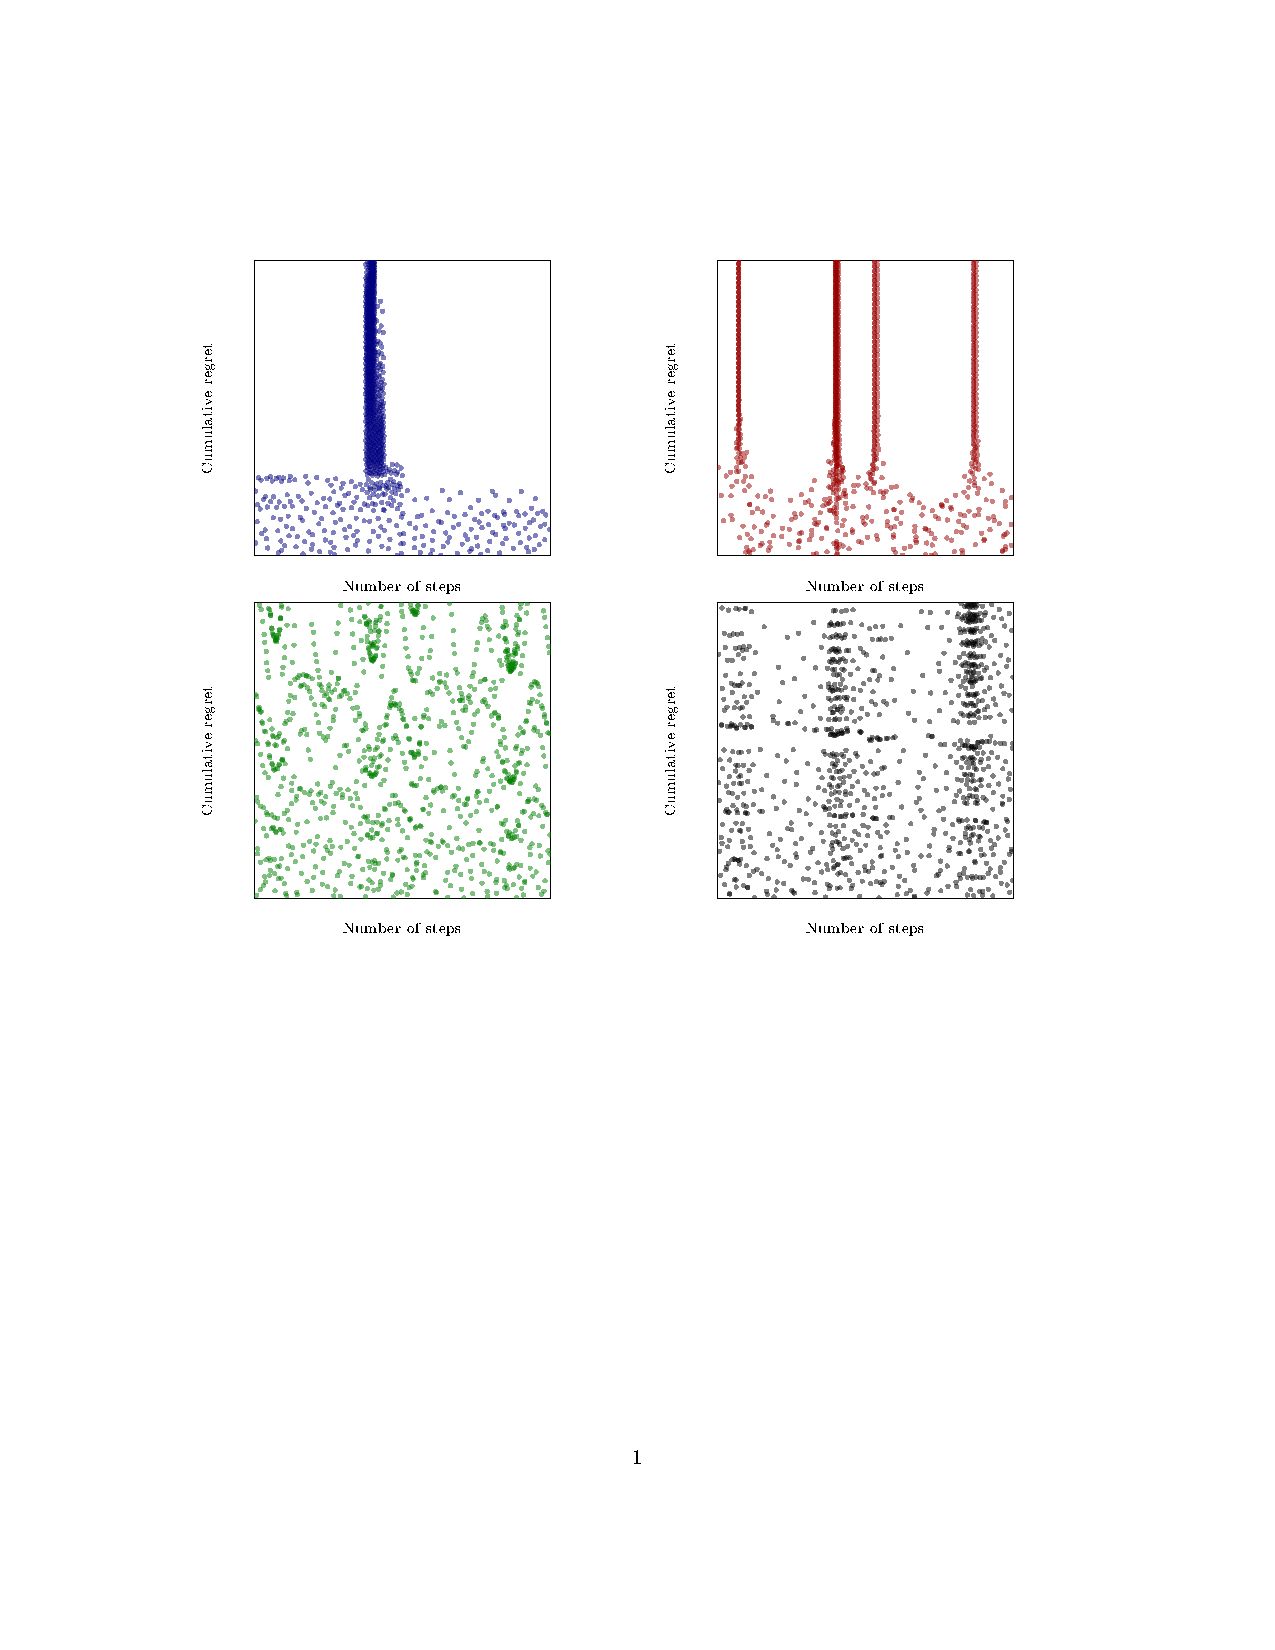
\includegraphics[trim = {0 6cm 0 4cm},clip]{marginal1000.pdf}
  \caption{Points sampled by the algorithms for Sinprod with 1000 evaluations. From top left to bottom right : HOO, POO, StoSOO and HCT. For this function, $x^*\simeq 0.86$ and the second best point is roughly in $0.39$.}
\end{figure}
%%%%%%%%%%%%%%%%%%%%%%%%%%% CUMULATIVE 1000 POINTS %%%%%%%%%%%%%%%%%%%%
\begin{figure}
\centering
\label{fig:cumulative1000}
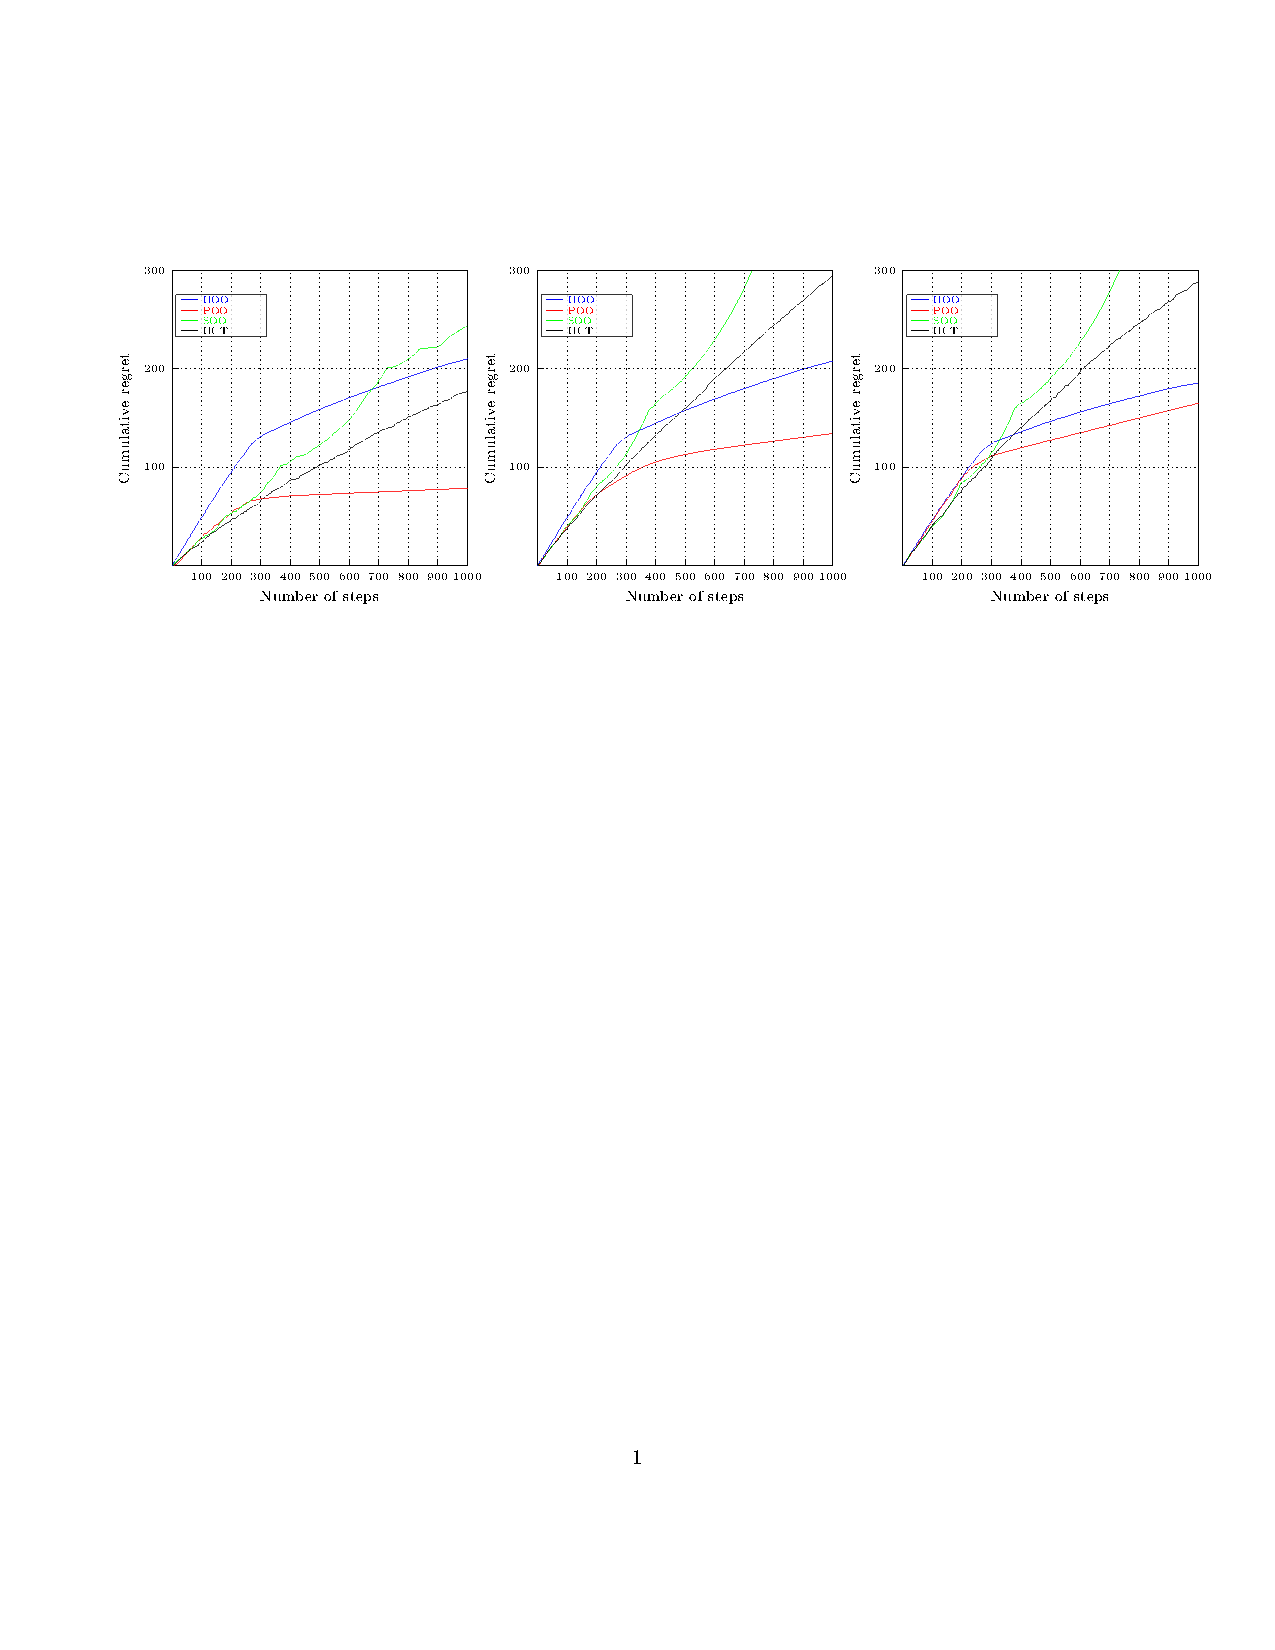
\includegraphics[trim={0 6cm 0 4cm},clip]{cumulative1000.pdf}
\caption{The cumulative regret of the 5 algorithms on the three difficult functions, with 1000 evaluations. From left to right : Grill function, Garland function, Sinprod function.}
\end{figure}

%%%%%%%%%%%%%%%%%%%%%%%%%%% NOISE = 0.1 %%%%%%%%%%%%%%%%%%%%
\begin{figure}
\centering
\label{fig:noise01}
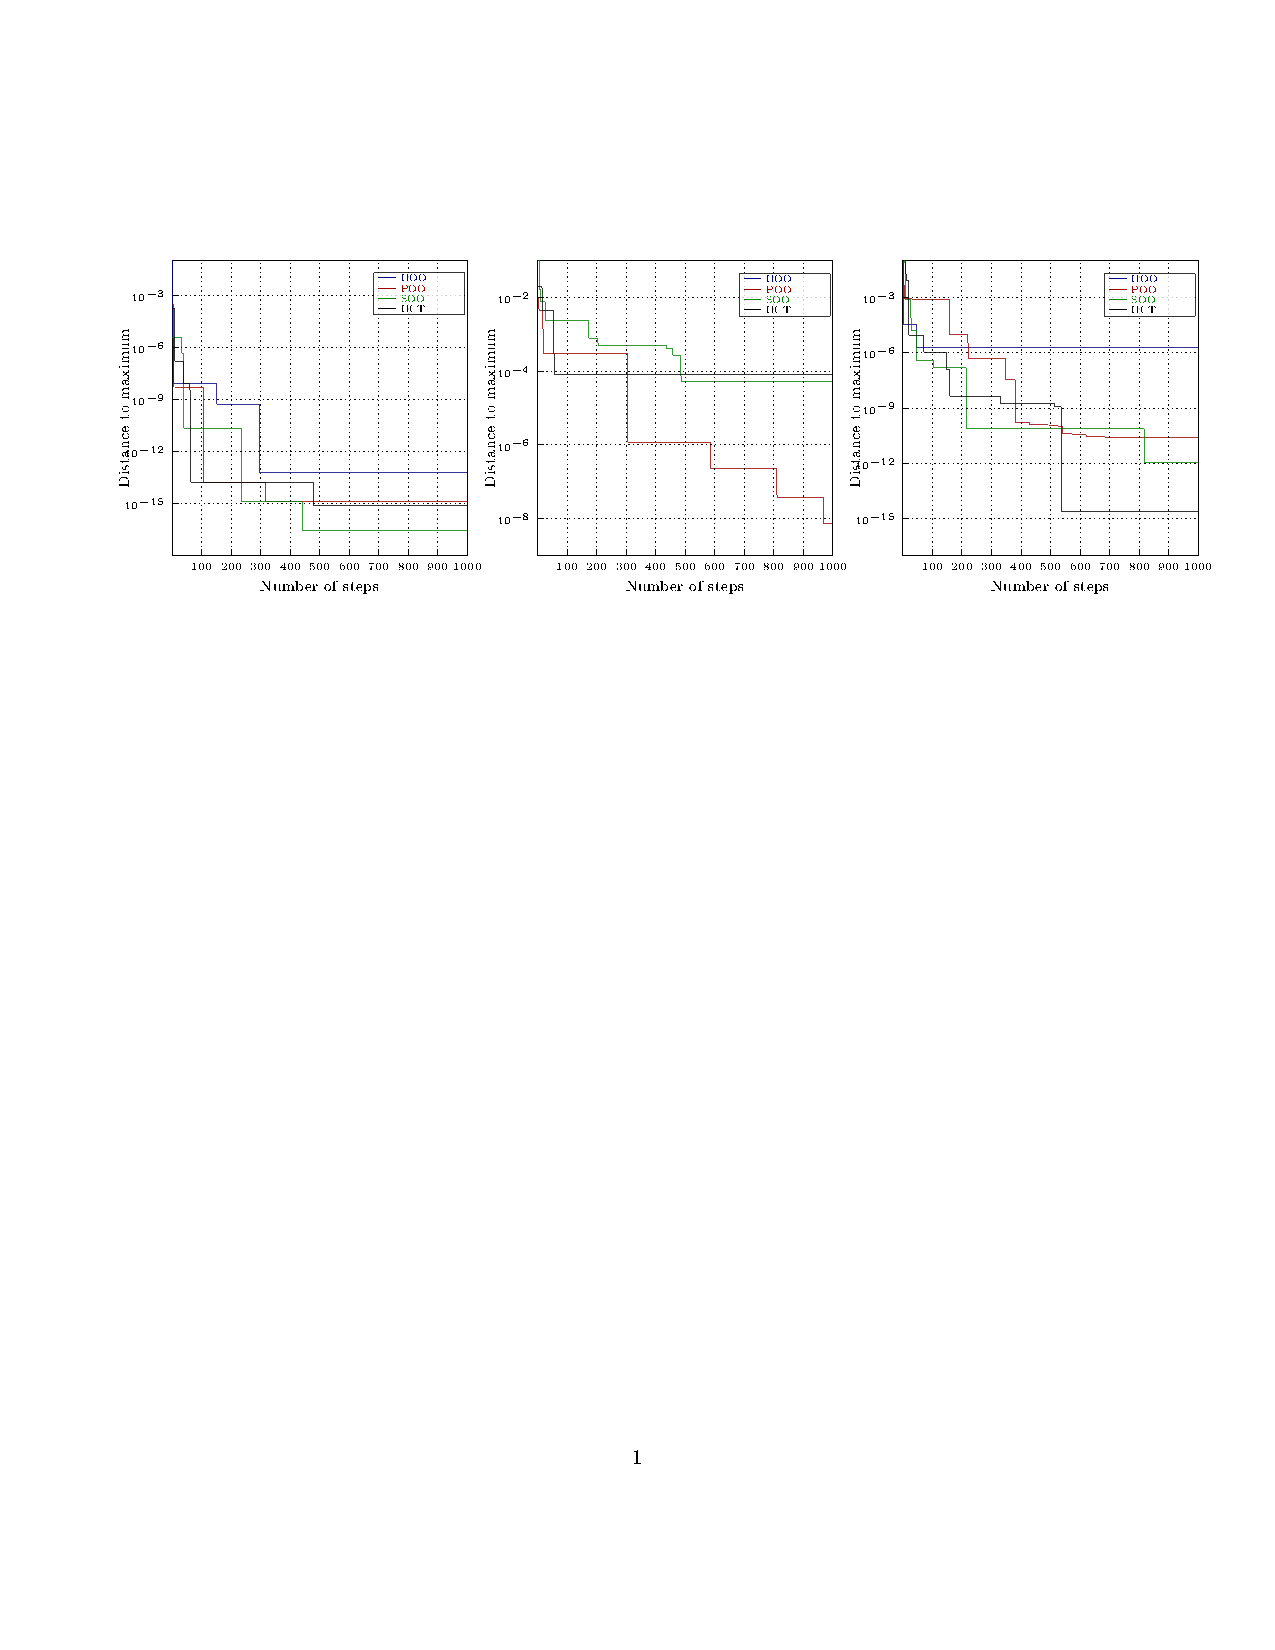
\includegraphics[trim={0 6cm 0 4cm},clip]{best1000_01.pdf}\\
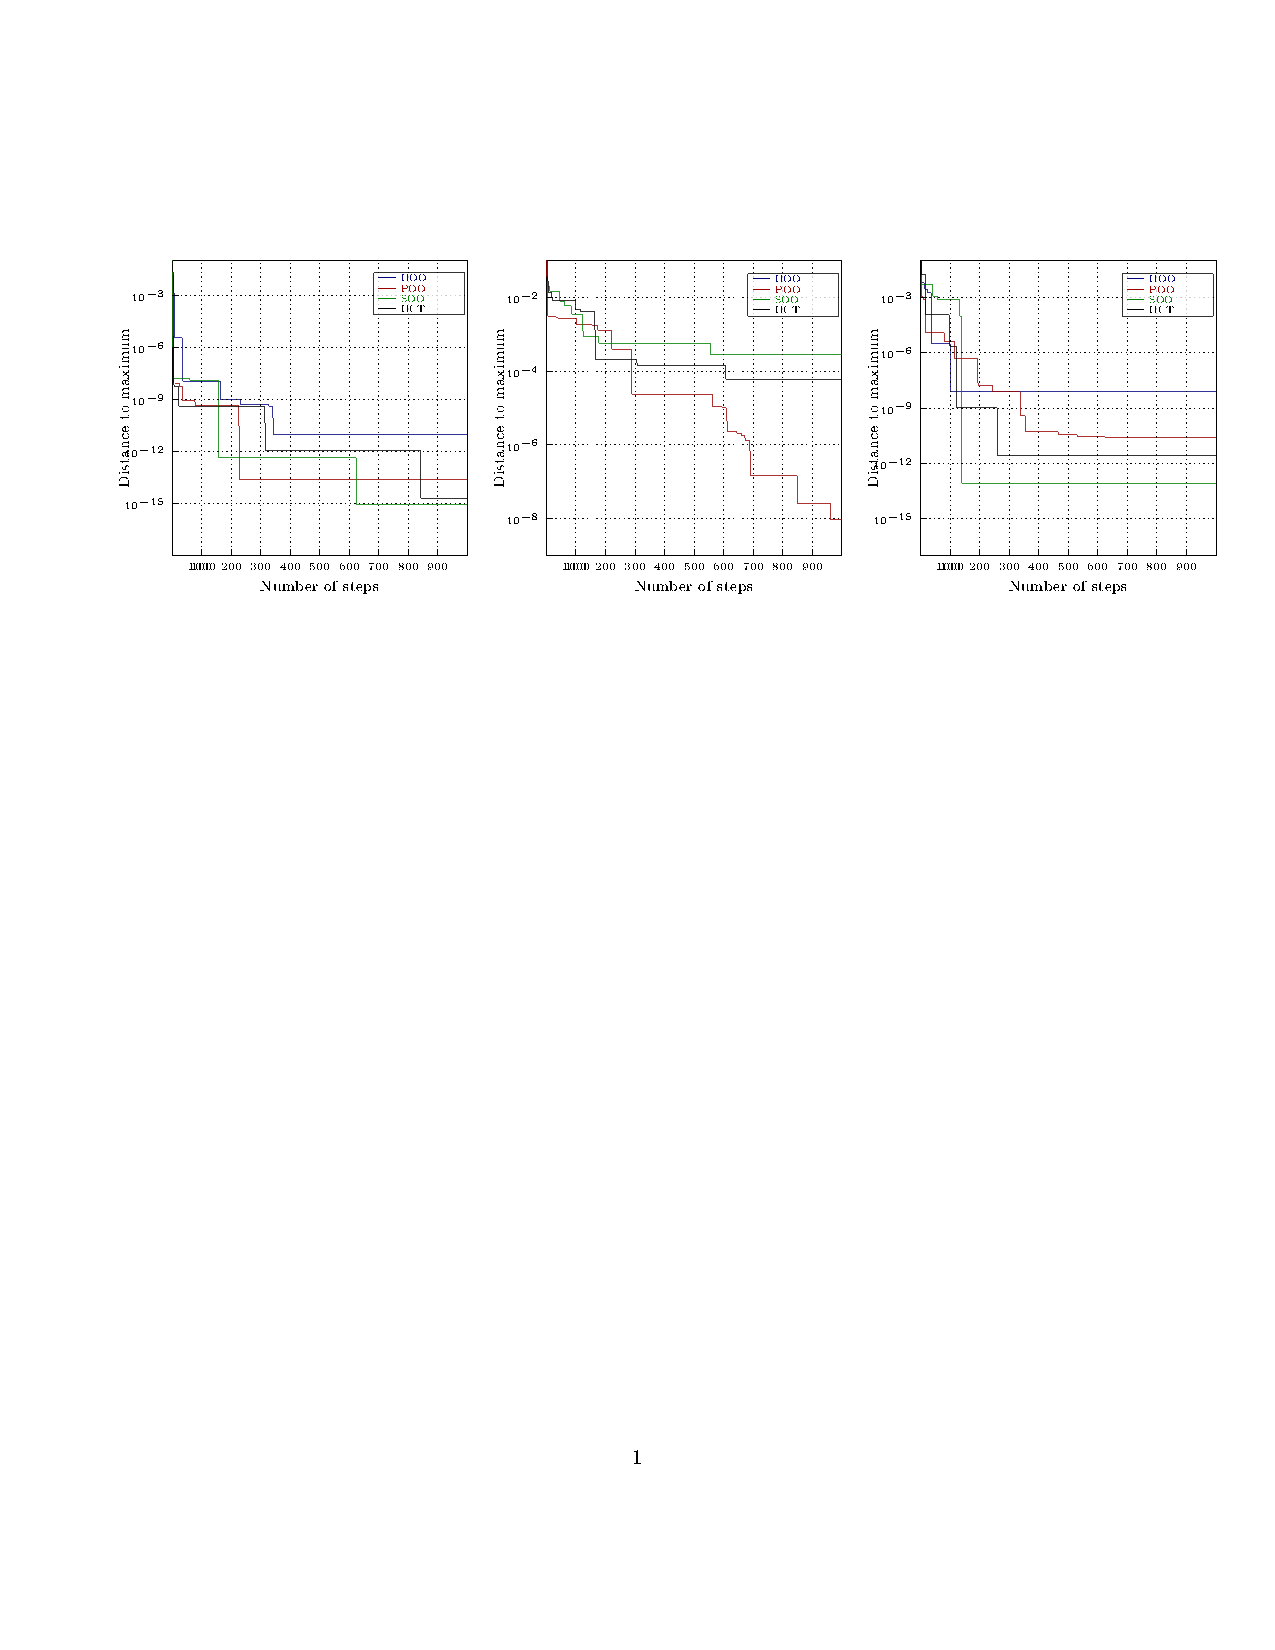
\includegraphics[trim={0 6cm 0 4cm},clip]{best1000_1.pdf}
 \caption{Best current regret under noisy estimation sampled from $\mathcal{N}(0,0.1)$ (top line) and $\mathcal{N}(0,1)$ (bottom line). From left to right : Grill function, Garland function, Sinprod function.}
\end{figure}

%%%%%%%%%%%%%%%%%%%%%%%%%%% ATB %%%%%%%%%%%%%%%%%%%%
\begin{figure}
\centering
\label{fig:atb}
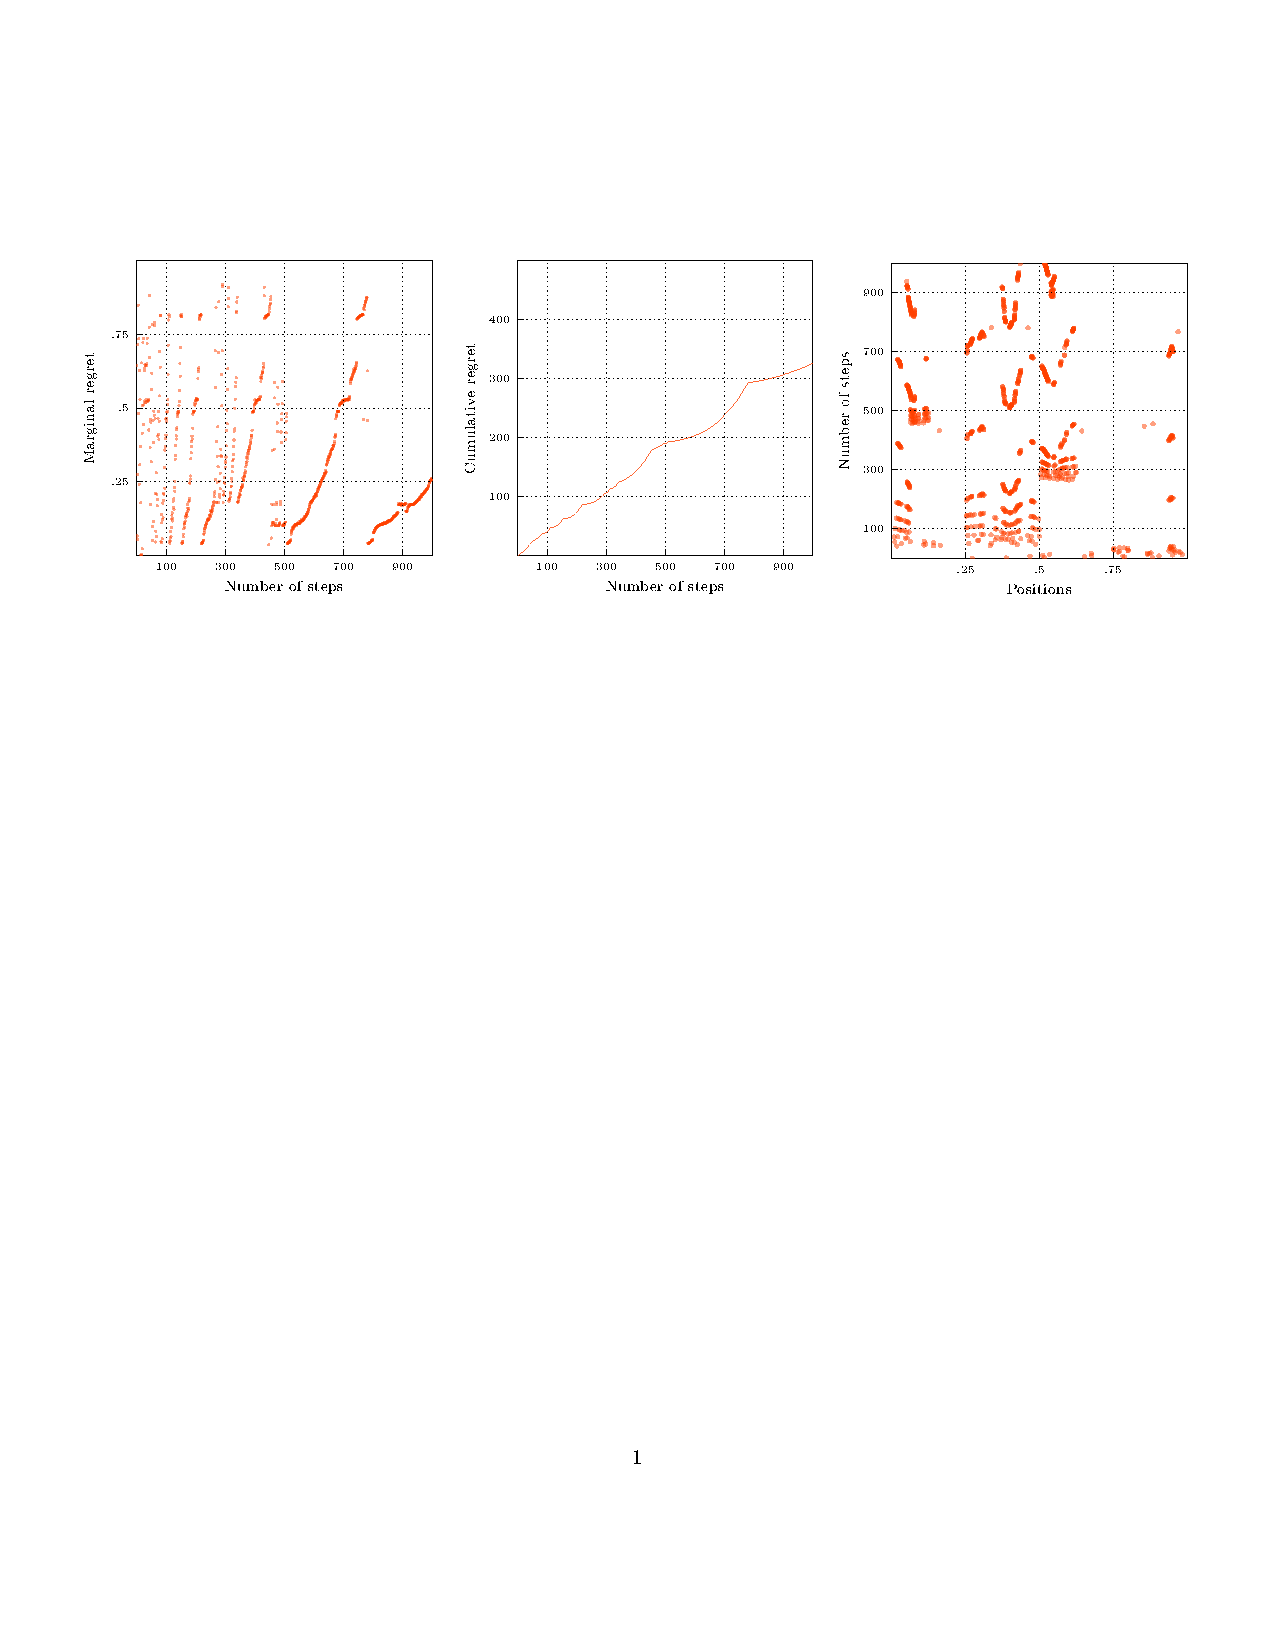
\includegraphics[trim={0 6cm 0 4cm},clip]{ATB.pdf}
\caption{From the left to the right: simple and cumulative regrets and sampled points for ATB algorithm on Sinprod optimization.}
\end{figure}
%%%% BIBILIOGRAPHY %%%%
\clearpage
\bibliographystyle{plain}
\bibliography{Biblio}{}
\nocite{*}

\label{lastpage}

\end{document}
